\subsection{closure test}
\begin{frame}{Geometric Interpretation}
    Consider 2 data points on an axis in the basis which diagonalises $C$ normalised by the square root of the eigenvalues:

    \begin{center}
        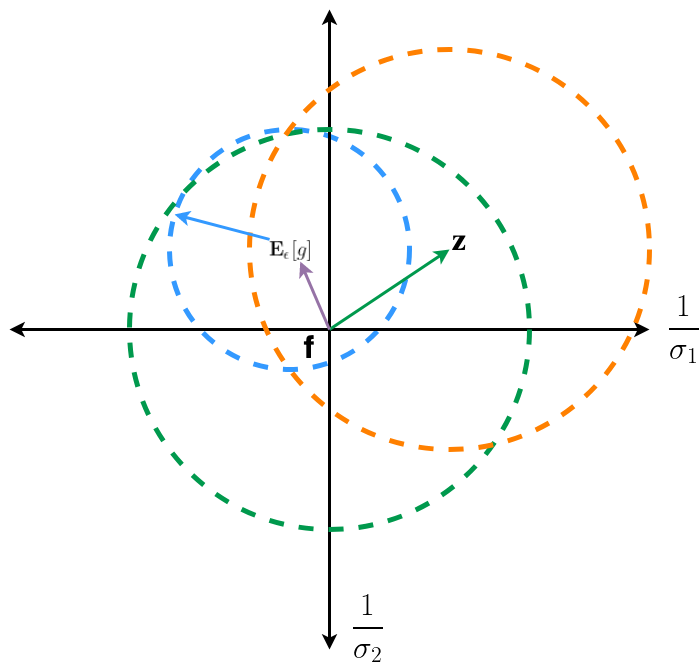
\includegraphics[scale=0.3]{closure_test/testdiaggram.png}
    \end{center}
\end{frame}
\begin{frame}{Statistical estimators - more detail}
    Decompose the expectation value of the likelihood function, $\chi^2$, by completing the square. Exposing some statistical indicators
    \begin{equation}
        \begin{split}
            \erep[\chi^2(g; y)] &= \frac{1}{\ndata}\erep[(\vv{g} - \vv{y})^T C^{-1} (\vv{g} - \vv{y})] \\
            &= {\rm bias} + {\rm variance} + {\rm noise} - {\rm cross term}
        \end{split}
    \end{equation}
    focus on the first two terms:
    \begin{equation}
        {\rm bias} = \frac{1}{\ndata}(\vv{f} - \erep[\vv{g}])^T C^{-1} (\vv{f} - \erep[\vv{g}])
    \end{equation}
    \begin{equation}
        {\rm variance} = \frac{1}{\ndata} \erep\left[ (\vv{g} - \erep[\vv{g}])^T C^{-1} (\vv{g} - \erep[\vv{g}]) \right]
    \end{equation}
    
    where $\erep[\cdot]$ is the expectation across replicas.
    
    \vspace{2pt}
    \begin{itemize}
        \item Faithful uncertainties if $(\vv{g} - \erep[\vv{g}])$ and $(\vv{f} - \erep[\vv{g}])$ have same distribution.
        \item Sample $(\vv{g} - \erep[\vv{g}])$ through sampling $\epsilon$ - usual MC replica procedure
        \item Sample $(\vv{f} - \erep[\vv{g}])$ distribution through sampling $\shift$ - only possible in closure test!
    \end{itemize}
\end{frame}
\begin{frame}[t]\frametitle{Preliminary results}
    Breakdown of $\eshift[{\rm bias}] / \eshift[{\rm variance}]$ for out of sample data by experiment - fitted on NNPDF3.1 dataset and validated on additional datasets to be included in NNDPF4.0

    \vspace{8pt}
    \begin{center}
    \begin{tabular}{lr}
        \toprule
        {} &  $\sqrt{\eshift[{\rm bias}] / \eshift[{\rm variance}]}$\\
        \midrule
        ATLAS      & 1.17 $\pm$ 0.4 \\
        CMS        & 1.07 $\pm$ 0.5 \\
        LHCb        & 0.83 $\pm$ 0.6 \\
        Total      & 1.11 $\pm$ 0.5 \\
        \bottomrule
        \end{tabular}
    \end{center}

\end{frame}